%%%%%%%%%%%%%%%%%%%%%%% file template-ljm.tex %%%%%%%%%%%%%%%%%%%%%%%%%
%
% This is a general template file for the LaTeX package ljm-auth
% for Lobachevskii Journal of Mathematics 2009/07/20
%
% Copy it to a new file with a new name and use it as the basis
% for your article. Delete % signs as needed.
%

%%%%%%%%%%%%%%%%%%%%%%%%%%%%%%%%%%%%%%%%%%%%%%%%%%%%%%%%%%%%%%%%%%%

\documentclass[12pt]{amsart}

\usepackage{ljm-auth}

\usepackage{graphicx}

\usepackage{cite}

\newtheorem{definition}{Definition}
\newtheorem{theorem}{Theorem}
\newtheorem{corollary}{Corollary}
\newtheorem{lemma}{Lemma}

\author{Strongin R.G., Gergel V.P., Barkalov K.A., Sysoyev A.V.}
\crauthor{Strongin, Gergel, Barkalov, Sysoyev} % for running heads

\tit{Generalized Parallel Computational Schemes for Time-Consuming Global Optimization}
\shorttit{Parallel Schemes for Global Optimization} %for running heads

\setcounter{page}{1}

\begin{document}

\maketit

\address{Lobachevsky State University of Nizhni Novgorod}

\email{gergel@unn.ru}


\abstract{This paper addresses computationally intensive global optimization problems, for solving of which the supercomputing systems with exaflops performance can be required. To overcome such computational complexity, the paper proposes the generalized parallel computational schemes, which may involve numerous efficient parallel algorithms of global optimization. The proposed schemes include various ways of multilevel decomposition of parallel computations to guarantee the computational efficiency of supercomputing systems with shared and distributed memory multiprocessors with thousands of processors to meet global optimization challenges.}

\notes{0}
{
%\subclass{} % 2010 Mathematical Subject Classification

\keywords{
global optimization, information-statistical theory, parallel computations, high-performance computing, supercomputing technologies
}

\thank{
This research was supported by the Russian Science Foundation, project No 16-11-10150 ``Novel efficient methods and software tools for time-consuming decision making problems using supercomputers of superior performance''
}
}


\section{Introduction}

Forthcoming exascale supercomputing systems with exaflops performance are intended to solve the computationally intensive problems with huge computational complexity. For an efficient use of the exascale supercomputers, the algorithms to solve such problems must be supreme parallel to utilize the great computational potential of millions of processors/nodes.

Undoubtedly, the global optimization problems arising in various areas of applications are computationally intensive ones, which may require the exascale supercomputing. These are the most complex problems of the theory and practice of optimal decision making. The optimized functions in these problems can be the multiextremal ones, i.e. can have numerous local optima with different values within the search domain. The multiextremality makes the optimization problems much more complicated as it requires the analysis of the entire feasible search domain. Even if the optimization problem dimensionality is small sufficiently, solving the global optimization problems requires a significant amount of computations (as few as several optimized variables can require the exascale supercomputing).

In addition, the global optimization problems are usual in the most difficult optimal decision making cases, i.e. during the computer-aided design of complex devices and systems. In the context of such problems, the performance criteria are nonlinear mostly, the search domains may be disconnected, and, above all, computing the function values may be computational intensive.

The state-of-the-art in the field of global optimization is outlined in a number of key works – see, for instance, \cite{Floudas, Locatelli, Strongin1, Pardalos, Sergeyev1, Paulavicius}. The development of the theory and methods of use of the high-performance computing for solving the computationally intensive problems of global optimization is one of the trends developing rapidly \cite{Strongin1, Ciegis, Luque, Strongin2}.

The present paper proposes generalized parallel computational schemes, which can be applied for constructing numerous efficient parallel algorithms of global optimization. The proposed schemes include various ways of multilevel decomposition of parallel computations to guarantee the computational efficiency of supercomputing systems with shared and distributed memory multiprocessors with thousands of processors to meet the global optimization challenges.

The rest of the paper has the following structure. Chapter 2 formulates the multidimensional problems of global optimization and describes an approach to the reduction of these ones to the one-dimensional optimization problems. Chapter 3 presents the generalized schemes of parallel computations for the supercomputing systems with shared and distributed memory multiprocessors. Chapter 4 presents the results of numerical experiments, which confirm the efficiency of the developed computational schemes. This is followed by the conclusions and potential ways of further research.


\section{Multidimensional problems of global optimization and their reduction}

A multidimensional global optimization problem can be stated as follows: to find a global minimum point $y^\ast \in R^N$ where the optimized function $\varphi(y)$ has the minimum value, i.e.
\begin{equation}
\varphi^\ast = \varphi(y^\ast) = \min \{\varphi(y): y\in D \},
\end{equation}
where $D$ is the search domain with given boundary vectors $a$ and $b$
\[
D=\left\{y\in R^N: a_i\leq y_i \leq b_i, 1\leq i \leq N\right\}.
\]
It is supposed that the objective function $\varphi(y)$ satisfies a Lipschitz condition
\begin{equation}
\vert \varphi(y') - \varphi(y'') \vert \leq L\| y' - y'' \|, \quad y', y'' \in D,
\end{equation}
where $L > 0$ is the Lipschitz constant, and $\|\ast\|$ is the Euclidian norm in the space $R^N$. Satisfying the Lipschitz condition is important as it allows estimating the global minimum on the basis of the finite number of computed values of the optimized function.

It is supposed also that the minimized function $\varphi(y)$ is defined by a computational procedure for computing the value $\varphi(y)$ at any point $y \in D$ (hereafter such computations will be called \textit{trials}). It should be pointed out that this procedure can be computationally intensive and, hence, the computational cost of solving the optimization problem (1) is determined mainly by the number of executed trials. 

As it is well known (see, for example, \cite{Strongin1}), the numerical evaluation of the global optimum points of the minimized functions requires constructing a coverage of the search domain $D$. This results in a very high computational intensity of global optimization problems even in the case of small dimensionality.

The computational complexity can be reduced considerably if the computational grids resulting from covering the search domain are non-uniform, i.e. when the grid nodes are distributed denser around the global optimal point only. The construction of such non-uniform coverings may be ensured in the case of an adaptive computation, when in order to select the new trial points, all search information obtained in the course of computation (previous trial points and the values of the minimized function at these points) is used. This necessary condition complicates the computational schemes of the global optimization methods essentially as it involves the computationally intensive analysis of large amounts of the multidimensional search information. As a result, many optimization algorithms use various dimensionality reduction schemes to certain extent (see, for example, \cite{Strongin1, Strongin2, Sergeyev2}).

In the framework of the information-statistical theory, the dimensionality reduction is provided by using the Peano space-filling curves $y(x)$, which map the interval $[0, 1]$ onto a $N$-dimensional domain $D$ \cite{Strongin1, Sergeyev2, Strongin3}. As a result of such reduction, the initial multidimensional global optimization problem (1) is reduced to a one-dimensional one:
\begin{equation}
\varphi(y(x^\ast)) = \min\{\varphi(y(x)): x \in [0,1]\}.
\end{equation}
for which the function $\varphi(y(x))$ satisfies a uniform H\"older condition \cite{Strongin1}, i.e.
\begin{equation}
|\varphi(y(x')-\varphi(y(x''))| \leq H|x' - x''|^{1/N}, x', x'' \in [0,1]\},
\end{equation}
where the H\"older constant $H$ is determined as $H = 2L\sqrt{N + 3}$, $L$ is the Lipschitz constant from (2) and $N$ is the optimization problem dimension (1). A one-dimensional function $\varphi(y(x))$ is produced by reduction of the multi-dimensional function $\varphi(y)$. In order to calculate the values of $\varphi(y(x))$, the multidimensional image $y \in D$ should be computed first in accordance with the mapping $y(x)$, and then the value of the multidimensional function $\varphi(y)$ at the multidimensional point $y \in D$ should be evaluated. The resulting value $z = \varphi(y)$ is used further as the value of the one-dimensional function $\varphi(y(x))$.


\section{Multilevel parallel computational schemes for solving computationally intensive global optimization problems}

The information-statistical theory proposes a general parallelization approach for solving the global optimization problems \textit{where parallelism is provided by simultaneous computations of the values for the minimized function $\varphi(y)$ at several different points in the search domain $D$} -- see, for example, \cite{Strongin1, Strongin2, Strongin4}. Such an approach ensures the parallelism of the most computationally intensive part of the global optimization and has a general nature as it is applicable to almost any global search method for solving any kind of global optimization problems.


\subsection{General computational scheme of global optimization algorithms}

The information-statistical theory \cite{Strongin1, Strongin3} formed a basis for many efficient global optimization methods -- see, for example \cite{Strongin2, Sergeyev4, Gergel1, Gergel2, Barkalov, Gergel3, Gergel4, Gergel5, Lera}. Moreover, a general computation scheme \cite{Strongin1, Strongin2, Strongin3, Grishagin1, Grishagin2} was proposed for all developed global search algorithms. This scheme can be represented as follows.

The initial global search algorithm iteration takes place at an arbitrary point $x^1 \in (0,1)$. Let then $k, k > 1$, global search iterations have been executed. Selection of the trial point ($k + 1$) for the next iteration is subject to the following rules.

\textit{Rule}~1. Renumber the previous iteration points by subscripts in the increasing order of coordinates
\begin{equation}
0 = x_0 < x_1 < \dots < x_i < \dots < x_k < x_{k+1} = 1,
\end{equation}
the points $x_0, x_{k+1}$ were added for convenience of further description.

\textit{Rule}~2. Compute a quantity $R(i)$ for each interval $(x_{i-1}, x_i), 1 \leq i \leq k + 1$ (hereafter, these quantities will be called \textit{characteristics}).

\textit{Rule}~3. Determine the interval with the maximum characteristic
\begin{equation}
R(t) = \max_{1 \leq i \leq k + 1}R(i).
\end{equation}

\textit{Rule} 4. Execute a new trial (compute the value of the minimized function $\varphi(y(x)))$ at the point $x^{k+1}$ in the interval with the maximum characteristic from (6).

The stopping condition to terminate the optimization iterations is defined by the inequality
\begin{equation}
(x_t - x_{t-1}) \leq \varepsilon,
\end{equation}
for the interval $t, 1 \leq i \leq k + 1$ with the maximum characteristic from (6) and $\varepsilon > 0$ is the required problem solving accuracy. If the stopping condition is not satisfied, the iteration number $k$ is incremented by unity, and a new global search iteration is executed.

The computed characteristics $R(i), 1 \leq i \leq k + 1$ can be understood as the importance indicators for the intervals with respect to the global minimum point location. This provides the explanation for the interval selection scheme for executing the next trial: the point of every next global search iteration is selected in the interval with the maximum characteristic (i.e. in the interval, which is the most likely one to contain the global minimum point).

According to this general scheme, specific global search algorithms are formulated by defining the formulas to compute the characteristics $R(i), 1 \leq i \leq k+1$, and the points of the next trials in the intervals with maximum characteristics. Thus, for a multidimensional general algorithm of global search (MGAGS) \cite{Strongin1}, the interval characteristic is defined as
\begin{equation}
R(i)=m\rho_i+\frac{(z_i-z_{i-1})^2}{m\rho_i}-2 (z_i + z_{i-1}), 1 \leq i \leq k + 1,
\end{equation}
where $m$ is the H\"older constant estimate from (4), $z_i = \varphi(y(x_i)), 1 \leq i \leq k + 1$ are the computed values of the minimized function $\varphi(y(x))$ at the points of the executed iterations, and $\rho_i = \left(x_i - x_{i-1} \right)^{1/N}, 1 \leq i \leq k + 1$.

The next trial point in the case of MGAGS is computed as follows:
\begin{equation}
x^{k+1} = \frac{x_t+x_{t-1}}{2} - \mathrm{sign}(z_t-z_{t-1})\frac{1}{2r}\left[\frac{\left|z_t-z_{t-1}\right|}{m}\right]^N,
\end{equation}
where $r, r > 1$ is a \textit{parameter} of the algorithm.

Additional information about the global optimization algorithms that can formulated in accordance with the described general computational scheme can be found in \cite{Strongin1, Strongin2}.


\subsection{Competitive parallel computational schemes for shared memory multiprocessors}

As it has been noted above, the general approach to provide the parallel computations consists in simultaneous calculating the minimized function values at several different points of the searching domain $D$. As the interval characteristics $R(i), 1 \leq i \leq k + 1$ (see Subsection 3.1) are understood as the importance indicators for the intervals with respect to the global minimum point location, additional intervals for several trials to be run in parallel should be selected subject to the following values of the characteristics.

As a result, a general scheme of the parallel algorithms of global optimization for systems with shared memory can be formulated on the basis of the scheme given in Subsection 3.1 where the following set of rules should be modified (see also \cite{Strongin1, Strongin2, Strongin4, Grishagin2}):

\textit{Rule} $3'$. Arrange the interval characteristics in the descending order
\begin{equation}
R(t_1) \geq R(t_2) \geq \dots \geq R(t_k) \geq R(t_{k+1})
\end{equation}
and select $p$ intervals with the numbers $t_j, 1 \leq j \leq p$ having the maximum values of characteristics ($p$ is the number of processors (cores) used for the parallel computing).

\textit{Rule} $4'$. Execute new trials (compute the values of the minimized function $\varphi(y(x))$) at the points $x^{k+j}, 1 \leq j \leq p$ located within the intervals with the maximum characteristics from (10).

The algorithm stopping condition (7) should be checked for all intervals where the trials are executed
\begin{equation}
\rho_{t_j} \leq \varepsilon, 1 \leq t_j \leq p.
\end{equation}
As it was mentioned above, if the stopping condition is not satisfied, the iteration number $k$ is incremented by $p$, and a new global search iteration should be executed.

In general, the described general scheme of parallel algorithms of global optimization for systems with shared memory identifies the procedure for competitive parallel computations (see Fig.~1a) where the search intervals $(x_{i-1} ,x_i), 1 \leq i \leq k + 1$ compete with each other for the access to the processors to execute next global search iterations. Taking into account the possible number of processors/cores in computational nodes with homogeneous shared memory, the described approach enables the parallelism of about $10^2$ computing units.

\begin{figure}[t]
\centering
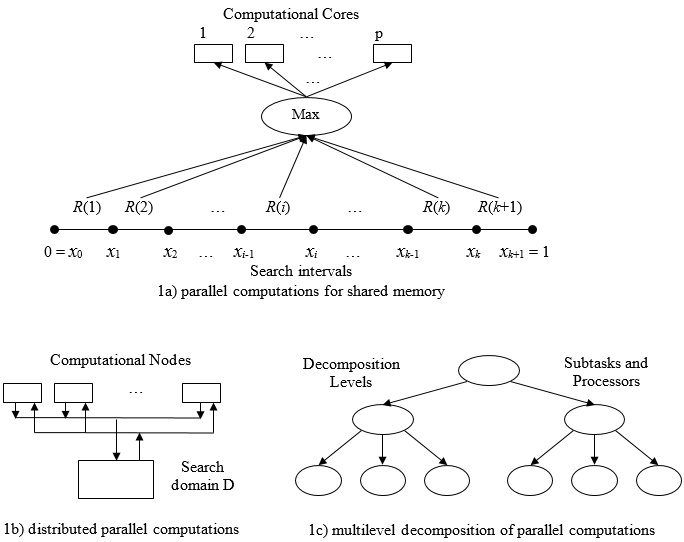
\includegraphics[width=13.0cm]{Fig1}
\caption{Generalized computational scheme of parallel algorithms}
\label{fig:Fig1}
\end{figure}

The conditions of convergence and nonredundancy of the resulting parallel computations for the global optimization algorithms formulated in the framework of general scheme of parallel algorithms of global optimization are given in \cite{Strongin1, Strongin2, Strongin4, Grishagin2}.


\subsection{Distributed parallel computations for high-performance systems}

The next level of parallel computations in the high-performance systems consists in the use of a number of computational nodes with distributed memory. A general approach can consist in the construction of a family of linked problems based on the initial global optimization problem (1)
\begin{equation}
\overrightarrow{\Phi} = \{ \phi_l(y), y \in D, 1 \leq l \leq s \},
\end{equation}
which can be solved in parallel using different computational nodes.

Generating such a family of problems can take place during the solving of the multicriterial optimization problems -- see, for example \cite{Gergel3, Gergel4}. Another approach used widely was proposed in \cite{Strongin1, Strongin2, Strongin5, Gergel1}. This approach uses a set of mappings
\begin{equation}
Y_s(x) = \{ y^1(x), \dots , y^s(x) \},
\end{equation}
allowing constructing the necessary family of optimization problems 
\begin{equation}
\phi\bigl(y^l(x^\ast_l)\bigr) = \min \bigl\{\phi\bigl(y^l(x)\bigl): x \in [0, 1] \bigl\}, 1 \leq l \leq s,
\end{equation}
for which the global minimum points coincide with the solution of the initial problem (1), i.e. $ y^\ast = y^l(x_l^\ast), 1 \leq l \leq s$. It is important to note that a family of the one-dimensional problems $\phi(y^l(x)), 1 \leq l \leq s$ resulting from the dimensionality reduction is an information-linked one: the function values computed for some function $\phi(yl(x))$ can be used by all other problems of the family (14).

Using such a parallelization approach can result in the following general scheme of parallel algorithms of global optimization for the systems with distributed and shared memory -- see also \cite{Gergel1} and Fig.~1b.

\begin{enumerate}
\item The family of one-dimensional reduced information-linked problems (14) is distributed among the computational nodes of high-performance system. One or more problems of the family $\overrightarrow{\Phi}(y)$ from (12) may be allocated to each separate node.

\item To solve the problems, each node uses the general scheme of parallel algorithms of global optimization for the system with shared memory described in Subsection 3.2 subject to the following rules of information interchange:

\begin{itemize}
\item Before starting a new trial for any problem $\phi(y^l(x)), 1 \leq l \leq s$ at any point $x' \in [0,1]$, it is necessary to calculate the image $y' \in D$ of the point $x' \in [0,1]$ according to the mapping of $y^l(x)$ and compute the preimages of $x_i', 1 \leq i \leq s$ for each problem of the family $\overrightarrow{\Phi}(y)$. The resulting preimages $x_i', 1 \leq i \leq s$ should be sent to all involved computational nodes to eliminate repeated selection of new trial points in the intervals containing the preimages.

\item Upon the completing of any trial for any problem $\phi(y^l(x)), 1 \leq l \leq s$ at any point $x' \in [0,1]$, calculate all preimages $x_i', 1 \leq i \leq s$ again and distribute these preimages and the trial result $z' = \phi(y^l(x'))$ among all involved computational nodes to include the obtained data in the search information (5).

\item Before starting the next global search iteration, the algorithm should accept the received data and include these ones into the search information (5).
\end{itemize}
\end{enumerate}

The described general scheme of parallel global optimization algorithms enables the parallel computing for the high-performance systems, which may contain many multiprocessor (multicore) computational nodes with the distributed memory. In addition, the computers may also include Intel Xeon Phi or GPGPU-based accelerators. Taking into account the required interchange of the optimization data, the estimated number of the computational nodes with distributed memory, which the proposed scheme allows to use efficiently makes up to $10^3-10^4$ (or total up to $10^5-10^6$ computational cores). 

The presented parallel computational scheme was discussed in \cite{Strongin1, Strongin2, Strongin5, Gergel1}.


\subsection{Multilevel decomposition of parallel computations for solving global optimization problems}

Further development of the parallel computations for solving the global optimization problems with the utilization of ever increasing number of processors/nodes can be ensured by integrating the computational scheme presented above with one more approach for the dimensionality reduction. This approach consists in a multistage decomposition scheme for the optimization problems \cite{Strongin2, Sergeyev4, Gergel5}. According to this scheme, a multidimensional global optimization problem can be reduced to a sequence of the nested one-dimensional problems:
\begin{equation}
\min \lbrace \varphi(y): y \in D \rbrace = \min_{a_1 \leq y_1 \leq b_1} \min_{a_2 \leq y_2 \leq b_2} ... \min_{a_N \leq y_N \leq b_N} \varphi(y).
\end{equation}

The multistage scheme (15) can be generalized for the integration with the dimensionality reduction scheme based on the Peano curves \cite{Sysoyev}. According to the generalized multistage block scheme, the vector of variables $y \in D$ of the global optimization problem (1) is considered to be a set of block variables
\[
y = (y_1, y_2, ..., y_N) = (u_1, u_2, ..., u_M)
\]
where the $i$-th block variable $u_i$ consists of the consecutive elements of the vector $y$, i.e.
\[
u_1 = (y_1, y_2, ..., y_{N_1}), \dots, 
u_M = (y_{N-N_M+1}, y_{N-N_M+2}, ..., y_N).
\]
where $N_1 + N_2 + \dots + N_M = N$.

Using new variables $u_i, 1 \leq i \leq M$, the basic relation of the multistage scheme (15) can be rewritten in the form
\begin{equation}
\min_{y \in D} \varphi(y) = \min_{u_1 \in D_1} \min_{u_2 \in D_2} ... \min_{u_M \in D_M} \varphi(y),
\end{equation}
where the subdomains $D_i, 1 \leq i \leq M$, are the projections of the initial search domain $D$ onto the subspaces corresponding to the variables $u_i,1 \leq i \leq M$. As a result, the nested subproblems of the multistage block scheme
\begin{equation}
\varphi_i(u_1,...,u_i) = \min_{u_{i+1} \in D_{i+1}} \varphi_{i+1}(u_1,...u_i,u_{i+1}), 1 \leq i \leq M - 1
\end{equation}
are the multidimensional ones and can be reduced using the Peano curves as before.

To enable the parallel computations, numerous nested optimization subproblems can be generated at once on each decomposition level for solving these ones in parallel \cite{Sergeyev7} (see Fig.~1c). The resulting number of parallel subproblems can be controlled using a predefined parallelization vector
\begin{equation}
\pi = (\pi_1, \pi_2, ..., \pi_M),
\end{equation}
where $\pi_i, 1 \leq i \leq M$, is the number of subproblems in the $(i+1)$-th decomposition level being solved in parallel. For the $M$-th level, $\pi_M$ means the number of parallel trials in the course of minimization of $\varphi_M(u_1,...,u_M) = \varphi_M(y_1,...,y_N)$ by the variable $u_M$  subject to the fixed values of $u_1, \dots, u_{M-1}$. Thus, the total number of the involved processors/cores equals to
\begin{equation}
\Pi = 1 + \sum_{i=1}^{M-1} \prod_{j=1}^i \pi_j.
\end{equation}

Using the proposed parallel implementation of the multistage block scheme finalizes constructing the generalized computational scheme of parallel global optimization algorithms. The developed approach provides the efficient use of all processors/nodes of the exascale supercomputers. Thus, for example, for 10 parallel subproblems at each stage of the multistage block scheme with 3 reduction levels (i.e. $\pi_i = 10, 1 \leq i \leq M, M = 3$) the possible number of computational units running simultaneously can be $p = \ \sim10^8-10^9$. 

\section{Results of computational experiments}

The computational experiments were performed using the Lobachevsky supercomputer at the State University of Nizhny Novgorod (operating system -- CentOS 6.4, supercomputer management system - SLURM). Each computational node had two 8-core Intel Sandy Bridge E5-2660 2.2 GHz CPUs, 64 GB RAM, and 3 NVIDIA Kepler K20Х graphic processors ($2\,688$ cores, 6 GB GDDR5 RAM). Intel C++ 14.0.2 was used to generate the executable program code. SDK CUDA Toolkit 6.0 was used to generate the applications for the graphic processors.

To carry out the computational experiments, the Globalizer system \cite{Sysoyev} was used. Its algorithms were based on the generalized scheme of parallel computations for solving global optimization problems described above.
 
The global optimization problems within the executed experiments were constructed by the GKLS-generator \cite{Gaviano}. This generator constructs the multiextremal optimization problems with predetermined properties such as the number of local minima, the global minimum point, the function value at this point, etc. In addition, this generator can construct two different types of the optimization problems, Simple (less difficult ones) and Hard (more difficult ones).

To obtain more reliable estimates of the parallelization efficiency, 100 test problems of global optimization were solved. The maximum allowed number of parallel iterations was $Kmax = 10\,000$.

The computational experiments involved the use of $p$ nodes of the Lobachevsky supercomputer, each node used three NVIDIA Kepler K20Х graphic accelerators. Thus, for $p = 32$, the number of GPU accelerators were 96, each having $2\,688$ CUDA cores (i.e. total $258\,048$ CUDA cores). Table 1 shows the Globalizer execution time, while Table 2 gives obtained parallel speedup with respect to the execution time for single computational node.

Additional computational results for the proposed generalized parallel computational scheme are given in \cite{Gergel1, Gergel2, Barkalov, Gergel3, Gergel4}. In addition, Globalizer was used also to solve various applied problems of global optimization -- see, for example, \cite{Modorskii, Gergel6}.

\begin{table}
	\caption{Average problem solving time using \textit{p} nodes}
	\label{tab:tab1}
	\center
	\begin{tabular}{|c|c|c|c|}
	\hline 
		Problem class & \parbox[c]{1.6cm}{ \centering p = 8 } & 
		\parbox[c]{1.6cm}{ \centering p = 16 } &
		\parbox[c]{1.6cm}{ \centering p = 32 } \\
	\hline 
		Simple &  2.04 & 1.50 & 0.47 \\
	\hline 
		Hard   & 11.51 & 5.53 & 0.54 \\
	\hline 
	\end{tabular}
\end{table}

\begin{table}
	\caption{Parallel speedup with respect to the execution time for single computational node}
	\label{tab:tab2}
	\center
	\begin{tabular}{|c|c|c|c|}
	\hline 
		Problem class & \parbox[c]{1.6cm}{ \centering p = 8 } & 
		\parbox[c]{1.6cm}{ \centering p = 16 } &
		\parbox[c]{1.6cm}{ \centering p = 32 } \\
	\hline 
		Simple & 25 & 34 & 109 \\
	\hline 
		Hard   & 5  & 9  & 96  \\
	\hline 
	\end{tabular}
\end{table}


\section{Conclusion}

The paper proposes a generalized computational scheme of parallel algorithms for solving global optimization problems, which require the exascale computations. The developed approach includes a competitive parallel computational scheme for the systems with shared memory, the distributed parallel computations based on using the multiple Peano curves for the dimensionality reduction, and the multilevel decomposition of the parallel computations for the exascale supercomputers. In addition, the supercomputers may include also Intel Xeon Phi or GPGPU-based accelerators. The proposed schemes ensure the computational efficiency of the supercomputing systems with shared and distributed memory with thousands of processors to address the global optimization challenges.

A number of development trends are relevant to evolve the research. Additional theoretical analysis of the proposed parallel computation scheme should be evaluated. Also, a spectrum of parallel global optimization algorithms, which can be implemented in the framework of the proposed computational scheme, should be studied. Besides, additional computational experiments involving a larger number of computational units should be carried out to evaluate the efficiency of parallel computations for solving computationally intensive global optimization problems adequately.


%%%%%%%%%%%%%%%%%%%%%%%%%%%%%%%%%%%%%%%%%%%%%%%%%%%%%%%%%%%%%%%%%%

\begin{thebibliography}{20}

\bibitem{Floudas}
C.~A.~Floudas and M.~P.~Pardalos, \textit{Recent advances in global optimization} (Princeton University Press, 2016).

\bibitem{Locatelli}
M.~Locatelli and F.~Schoen, \textit{Global optimization: theory, algorithms and applications} (SIAM, 2013).

\bibitem{Strongin1}
R.~G.~Strongin and Y.~D.~Sergeyev, \textit{Global optimization with non-convex constraints. Sequential and parallel algorithms} (Kluwer Academic Publishers, Dordrecht, 2000, 2nd ed. 2013, 3rd ed. 2014).

\bibitem{Pardalos}
P.~M.~Pardalos, A.~A.~Zhigljavsky and J.~\v{Z}ilinskas \textit{Advances in stochastic and deterministic global optimization} (Springer, 2016).

\bibitem{Sergeyev1}
Y.~D.~Sergeyev and D.~E.~Kvasov, \textit{Deterministic Global Optimization. An Introduction to the Diagonal Approach}  (Springer Briefs in Optimization, Springer, 2017).

\bibitem{Paulavicius}
R.~Paulavi\v{c}ius, J.~\v{Z}ilinskas, \textit{Simplicial Global Optimization} (Springer Briefs in Optimization. Springer, 2014).

\bibitem{Ciegis}
R.~\v{C}iegis, D.~Henty, B.~K\r{a}gstr\"om and J.~\v{Z}ilinskas, \textit{Parallel scientific computing and optimization: advances and applications}  (Springer, 2009). 

\bibitem{Luque}
G.~Luque and E.~Alba, \textit{Parallel genetic algorithms. Theory and real world applications} (Springer-Verlag, Berlin, 2011).

\bibitem{Strongin2}
R.~G.~Strongin, V.~P.~Gergel, V.~A.~Grishagin and K.~A.~Barkalov, \textit{Parallel computations for global optimization problems} (Moscow State University, Moscow, 2013) [In Russian].

\bibitem{Sergeyev2}
Ya.~D.~Sergeyev, R.~G.~Strongin, D.~Lera, \textit{Introduction to Global Optimization Exploiting Space-Filling Curves} (Springer Briefs in Optimization, Springer, 2013).

\bibitem{Strongin3}
R.~G.~Strongin, \textit{Numerical Methods in Multiextremal Problems (Information-Statistical Algorithms)} (Nauka, Moscow, 1978) [In Russian].

\bibitem{Strongin4}
R.~G.~Strongin and Y.~D.~Sergeyev, \textit{Global multidimensional optimization on parallel computer}, Parallel Computing, \textbf{18} (11), 1259--1273, (1992).

\bibitem{Sergeyev4}
Y.~D.~Sergeyev and V.~A.~Grishagin, \textit{Parallel asynchronous global search and the nested optimization scheme}, J. Comput. Anal. Appl., \textbf{3} (2), 123--145, (2001).

\bibitem{Gergel1}
V.~P.~Gergel and S.~V.~Sidorov, \textit{A Two-Level Parallel Global Search Algorithm for Solution of Computationally Intensive Multiextremal Optimization Problems}, V. Malyshkin (Ed.): PaCT 2015, LNCS 9251, 505--515. Springer-Verlag Berlin Heidelberg ,(2015).

\bibitem{Gergel2}
V.~Gergel, \textit{An Unified Approach to Use of Coprocessors of Various Types for Solving Global Optimization Problems}, 2nd International Conference on Mathematics and Computers in Sciences and in Industry, 13--18, (2015).

\bibitem{Barkalov}
K.~Barkalov, V.~Gergel and I.~Lebedev, \textit{Solving global optimization problems on GPU cluster}, In: Simos, T.E. (ed.) ICNAAM 2015. AIP Conference Proceedings, 1738, art. no. 400006, (2016).

\bibitem{Gergel3}
V.~Gergel and E.~Kozinov, \textit{Efficient methods of multicriterial optimization based on the intensive use of search information}, Springer Proceedings in Mathematics and Statistics, 197, 27--45, (2017). 

\bibitem{Gergel4}
V.~Gergel and E.~Kozinov, \textit{Parallel computing for time-consuming multicriterial optimization problems}, Lecture Notes in Computer Science, 10421, 446--458, (2017).

\bibitem{Gergel5}
V.~Gergel, V.~Grishagin and A.~Gergel, \textit{Adaptive nested optimization scheme for multidimensional global search}, Journal of Global Optimization, \textbf{66} (1), 35--51, (2016).

\bibitem{Lera}
D.~Lera, Y.~D.~Sergeyev, \textit{Lipschitz and Holder global optimization using space-filling curves}, Appl. Numer. Math, \textbf{60} (1-2), 115--129, (2010).

\bibitem{Grishagin1}
V~A.~Grishagin, \textit{On convergence conditions for a class of global search algorithms}, Proceedings of the 3-rd All-Union seminar ``Numerical methods of nonlinear programming'', Kharkov, 82--84, (1979) [In Russian].

\bibitem{Grishagin2}
V.~A.~Grishagin, Y.~D.~Sergeyev and R.~G.~Strongin, \textit{Parallel characteristic algorithms for solving problems of global optimization}, Journal of Global Optimization, \textbf{10} (2), 185--206, (1997).

\bibitem{Strongin5}
R.~G.~Strongin, \textit{Algorithms for Multi-extremal Mathematical Programming Problems Employing the Set of Joint Space-filling Curves}, Journal of Global Optimization, \textbf{2} (4), 357--378, (1992).

\bibitem{Sysoyev}
A.~Sysoyev, K.~Barkalov, V.~Sovrasov, I.~Lebedev and V.~Gergel, \textit{Globalizer –- A parallel software system for solving global optimization problems}, Lecture Notes in Computer Science 10421, 492--499, (2017). 

\bibitem{Sergeyev7}
Y.~D.~Sergeyev and V.~A.~Grishagin, \textit{Parallel Asynchronous Global Search and the Nested Optimization Scheme}, J. Comput. Anal. Appl., \textbf{3} (2), 123--145, (2001).

\bibitem{Gaviano}
M.~Gaviano, D.~Lera, D.~E.~Kvasov and Ya.~D.~Sergeyev, \textit{Software for generation of classes of test functions with known local and global minima for global optimization}, ACM Trans. Math. Software, \textbf{29}, 469--480, (2003).

\bibitem{Modorskii}
V.~Y.~Modorskii, D.~F.~Gaynutdinova, V.~P.~Gergel and K.~A.~Barkalov, \textit{Optimization in design of scientific products for purposes of cavitation problems}, AIP Conference Proceedings, 1738, art. no. 400013, (2016).

\bibitem{Gergel6}
V.~P.~Gergel, M.~I.~Kuzmin, N.~A.~Solovyov and V.~A.~Grishagin, \textit{Recognition of surface defects of cold-rolling sheets based on method of localities}, International Review of Automatic Control, \textbf{8} (1), 51--55, (2015).

\end{thebibliography}

\end{document}
